\section{}
\[
H(s)=\frac{s^2+4}{s\,(s^2+10s+100)}\,.
\]
\subsection{Bode-Diagramm}
\begin{center}
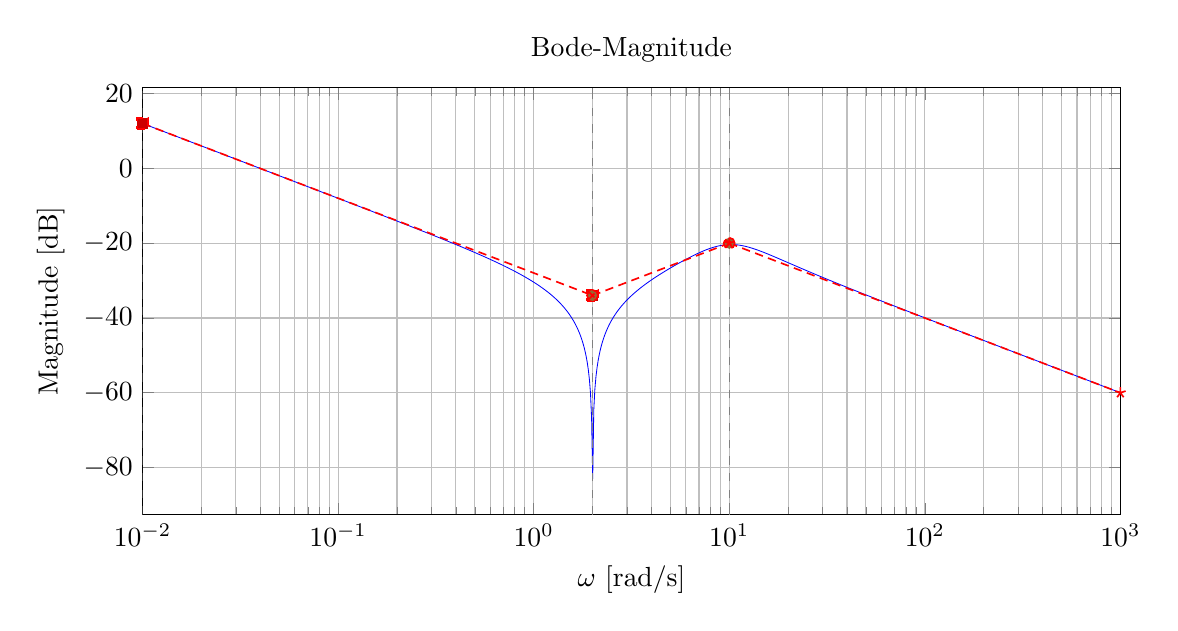
\begin{tikzpicture}
\begin{semilogxaxis}[
  width=14cm,height=7cm,
  xmin=1e-2,xmax=1e3,
  ytick distance=20,
  xlabel={$\omega$ [rad/s]},
  ylabel={Magnitude [dB]},
  grid=both,
  title={Bode-Magnitude}
]
\addplot[
  domain=1e-2:1e3,
  samples=900,
  mark=none,
  line width=0.3pt,
  blue
] {20*ln(abs(4 - x^2))/ln(10) - 20*ln(x)/ln(10) - 10*ln((100 - x^2)^2 + (10*x)^2)/ln(10)};
\addplot+[domain=1e-2:2,samples=2,dashed,dash pattern=on 3pt off 2pt,line width=0.6pt,red] {20*ln(0.04)/ln(10) - 20*ln(x)/ln(10)};
\addplot+[domain=2:1e1,samples=2,dashed,dash pattern=on 3pt off 2pt,line width=0.6pt,red] {-40 + 20*ln(x)/ln(10)};
\addplot+[domain=1e1:1e3,samples=2,dashed,dash pattern=on 3pt off 2pt,line width=0.6pt,red] {-20 - 20*ln(x/10)/ln(10)};
\draw[gray,dashed] (rel axis cs:0,0) -- (rel axis cs:0,1);
\draw[gray,dashed] (axis cs:2,\pgfkeysvalueof{/pgfplots/ymin}) -- (axis cs:2,\pgfkeysvalueof{/pgfplots/ymax});
\draw[gray,dashed] (axis cs:10,\pgfkeysvalueof{/pgfplots/ymin}) -- (axis cs:10,\pgfkeysvalueof{/pgfplots/ymax});
\node[gray,anchor=south east] at (axis cs:2,\pgfkeysvalueof{/pgfplots/ymax}) {\scriptsize Doppelnullstellen $\omega_z=2$ (j-Achse)};
\node[gray,anchor=south east] at (axis cs:10,\pgfkeysvalueof{/pgfplots/ymax}) {\scriptsize Polpaar $\omega_n=10$, $\zeta=0.5$};
\end{semilogxaxis}
\end{tikzpicture}
\vspace{6mm}
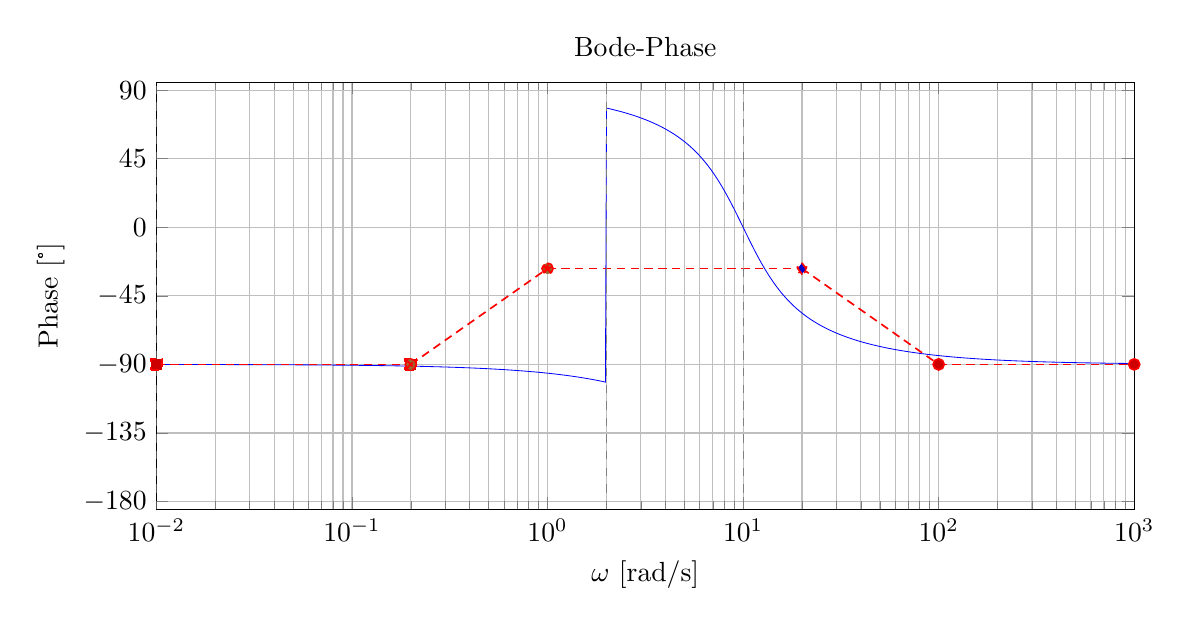
\begin{tikzpicture}
\begin{semilogxaxis}[
  width=14cm,height=7cm,
  xmin=1e-2,xmax=1e3,
  ytick distance=45,
  ymin=-185,ymax=95,
  xlabel={$\omega$ [rad/s]},
  ylabel={Phase [°]},
  grid=both,
  title={Bode-Phase}
]
\addplot[
  domain=1e-2:1e3,
  samples=900,
  mark=none,
  line width=0.3pt,
  blue
] {atan2(0, 4 - x^2) - 90 - atan2(x/10, 1 - (x/10)^2)};
\addplot+[domain=1e-2:2e-1,samples=2,dashed,dash pattern=on 3pt off 2pt,line width=0.6pt,red] {-90};
\addplot+[domain=2e-1:1e0,samples=2,dashed,dash pattern=on 3pt off 2pt,line width=0.6pt,red] {-90 + 90*ln(x/0.2)/ln(10)};
\addplot+[domain=1e0:2e1,samples=2,dashed,dash pattern=on 3pt off 2pt,line width=0.6pt,red] {-90 + 90*ln(5)/ln(10)};
\addplot+[domain=2e1:1e2,samples=2,dashed,dash pattern=on 3pt off 2pt,line width=0.6pt,red] {90 - 90*ln(x)/ln(10)};
\addplot+[domain=1e2:1e3,samples=2,dashed,dash pattern=on 3pt off 2pt,line width=0.6pt,red] {-90};
\draw[gray,dashed] (rel axis cs:0,0) -- (rel axis cs:0,1);
\draw[gray,dashed] (axis cs:2,\pgfkeysvalueof{/pgfplots/ymin}) -- (axis cs:2,\pgfkeysvalueof{/pgfplots/ymax});
\draw[gray,dashed] (axis cs:10,\pgfkeysvalueof{/pgfplots/ymin}) -- (axis cs:10,\pgfkeysvalueof{/pgfplots/ymax});
\node[gray,anchor=south east] at (axis cs:2,\pgfkeysvalueof{/pgfplots/ymax}) {\scriptsize Doppelnullstellen $\omega_z=2$ (j-Achse)};
\node[gray,anchor=south east] at (axis cs:10,\pgfkeysvalueof{/pgfplots/ymax}) {\scriptsize Polpaar $\omega_n=10$, $\zeta=0.5$};
\end{semilogxaxis}
\end{tikzpicture}
\end{center}
\newpage
\subsection{Erklärung}
\vspace{5mm}
\begin{description}[leftmargin=1.2em,labelsep=.6em,font=\bfseries]
\item[Schritt 1] Struktur: Integrator $1/s$, konjugiertes Polpaar mit $\omega_n=10$, $\zeta=0.5$, und Doppelnullen auf der j-Achse bei $\omega_z=2$. Für $\omega\ll2$: $|H(\j\omega)|\approx \dfrac{4}{100\,\omega}=0.04/\omega$ $\Rightarrow$ Slope $-20\,\mathrm{dB/dec}$ um Niveau $20\log_{10}0.04\approx-27.96\,\mathrm{dB}$ bei $\omega=1$; Phase $\approx-90^\circ$.
\item[Schritt 2] Doppelnullen bei $\omega_z=2$: Betrag hat dort ein exaktes Null ($|H(\j2)|=0$). Asymptotisch steigt die Slope hinter $\omega=2$ um $+40\,\mathrm{dB/dec}$ (Netto $-20\to+20\,\mathrm{dB/dec}$). Phasenbeitrag der Zählerdoppelnull ist exakt ein Sprung um $+180^\circ$ (von $0^\circ$ auf $180^\circ$); in der Geradennäherung als $+180^\circ$ über zwei Dekaden $[0.2,20]$ modelliert.
\item[Schritt 3] Polpaar bei $\omega_n=10$, $\zeta=0.5$: ab $\omega=10$ Slope-Änderung $-40\,\mathrm{dB/dec}$ (Netto $+20\to-20\,\mathrm{dB/dec}$). Exakt bei $\omega=10$: $|H(\j10)|=\dfrac{|4-100|}{10\cdot100}=\dfrac{96}{1000}\approx-20.35\,\mathrm{dB}$ (nahe der $-20\,\mathrm{dB}$-Asymptote). Phasenbeitrag des Polpaares $-180^\circ$ über $[1,100]$, wodurch die Gesamtsumme nach dem temporären Anheben durch die Zählernullen wieder gegen $\,-90^\circ$ fällt.
\end{description}

\vspace{0.5cm}
\medskip
\noindent\textbf{Stückweise Näherung}
\[
|H(\j\omega)|_{\mathrm{dB}}\approx
\begin{cases}
20\log_{10}(0.04)-20\log_{10}\omega,& \omega\ll2,\\[4pt]
-\infty,& \omega=2,\\[4pt]
-40+20\log_{10}\omega,& 2\ll\omega\ll10,\\[4pt]
-20-20\log_{10}(\omega/10),& \omega\gg10,
\end{cases}
\qquad
\]
\newpage